\documentclass[12pt, a4paper]{article}
\usepackage[utf8]{inputenc}
\usepackage{geometry}
\geometry{margin=1.25in}
\usepackage{graphicx}
\usepackage{caption}
\usepackage{subcaption}
\usepackage{booktabs}
\usepackage{amsmath}
\usepackage{hyperref}
\usepackage{tocloft}
\usepackage{lipsum} % For placeholder text, remove in final version
\usepackage{enumitem}


\title{Binary Classification of Lung Ultrasound Images for COVID-19 vs. Pneumonia}
\author{
\\
\\
\\

\includegraphics[width=6cm]{img/emblem.png}\\[2cm]
    \textbf{Abhijith C} \\
    Department of Computer Science and Engineering \\
    National Institute of Technology Karnataka (NITK) \\ 
    Surathkal, India \\
    Roll Number: 242CS003 \\ 
    Email: \href{mailto:abhijithc.242cs003@nitk.edu.in}{abhijithc.242cs003@nitk.edu.in}\\[0.5cm]
}
\date{}

\begin{document}

\maketitle
\newpage
\tableofcontents

\newpage
\begin{abstract}
This report presents a comprehensive study on the binary classification of lung ultrasound (LUS) images to distinguish COVID-19 from pneumonia. A literature survey was conducted to explore algorithms for LUS image classification, followed by experiments using three pretrained models: ResNet-50, VGG16, and Swin Tiny Transformer. Experiments were performed under four conditions: a balanced dataset, an imbalanced dataset, k-fold cross-validation, and grayscale images. Results are evaluated using accuracy, precision, recall, and F1-score, with a comparative analysis highlighting model performance across setups.
\end{abstract}

\section{Introduction}
\label{sec:introduction}
Lung ultrasound (LUS) has emerged as a valuable, non-invasive, portable, and cost-effective imaging modality for diagnosing pulmonary conditions such as pneumonia, COVID-19, and other lung abnormalities. The classification of LUS images involves identifying specific artifacts—such as A-lines, B-lines, consolidations, and pleural alterations—that indicate varying degrees of lung pathology. Due to challenges in manual interpretation, including operator dependency and image variability, automated classification algorithms, particularly those leveraging deep learning, have gained significant attention. This project aims to evaluate pretrained deep learning models for the binary classification of LUS images, comparing their performance across various dataset configurations.

This report is organized as follows: Section~\ref{sec:literature} reviews related work, Section~\ref{sec:methodology} details the methodology, Section~\ref{sec:results} presents experimental results, Section~\ref{sec:comparison} compares findings, Section~\ref{sec:discussion} discusses implications, and Section~\ref{sec:conclusion} concludes the study.

\section{Literature Survey}
\label{sec:literature}



\subsection{Challenges in Manual Interpretation of LUS Images}

Manual LUS interpretation faces several challenges:
\begin{itemize}
\item \textbf{Image Quality}: Speckle noise and artifacts reduce clarity \cite{vafaeezadeh}.
\item \textbf{Operator Dependency}: Results vary with the clinician’s experience \cite{vafaeezadeh}.
\item \textbf{Variability}: Differences in ultrasound devices and patient conditions complicate standardization \cite{diaz}.
\item \textbf{Data Scarcity}: Limited annotated datasets hinder robust model training \cite{vafaeezadeh}.
\end{itemize}
These issues underscore the need for automated algorithms that can generalize across diverse settings and provide reliable, reproducible diagnoses.

\subsection{Traditional Approaches: CNN-Based Classification of LUS}

CNNs have been the cornerstone of early automated LUS classification due to their ability to extract local features through convolutional layers.

\textbf{Diaz-Escobar \textit{et al.}}\cite{diaz}  evaluated VGG19, InceptionV3, Xception, and ResNet50 for classifying LUS images from the POCUS dataset (3326 frames: 1283 COVID-19, 731 pneumonia, 1312 healthy). The study used a 5×5-fold cross-validation approach, achieving the following results:
\begin{itemize}
  \item \textbf{InceptionV3}: Best performance with 89.1\% accuracy, 89.3\% balanced accuracy, and 97.1\% AUC-ROC.
   \item \textbf{Xceptio}: Close second with 88.6\% accuracy, 88.7\% balanced accuracy, and 96.8\% AUC-ROC.
   \item \textbf{POCOVID-net (VGG16-based)}: Baseline model with 86.5\% accuracy and 86.3\% balanced accuracy.
   \item \textbf{VGG19}: 85.8\% accuracy and 85.8\% balanced accuracy.
   \item \textbf{ResNet50}: Lowest at 78.3\% accuracy and 78.1\% balanced accuracy.
\end{itemize}

\textbf{Mascarenhas \textit{et al.}} \cite{mascarenhas} compared these architectures on a retail product classification task (6000 images, 5 classes). While not LUS-specific, their findings provide general insights:
\begin{itemize}
  \item \textbf{ResNet50}: Achieved the highest test accuracy (97.33\% at epoch 20).
  \item \textbf{VGG19}: 97.07\% test accuracy.
  \item \textbf{VGG16}: 96.67\% test accuracy.
\end{itemize}
  ResNet50’s residual connections likely enhance its ability to handle deeper networks, a trait potentially beneficial for complex LUS patterns, though its underperformance in \cite{diaz} suggests task-specific optimization is key. CNNs excel at local feature detection, are well-established with pre-trained models (e.g., ImageNet), and have demonstrated high accuracy in LUS classification \cite{diaz}. However, they struggle with long-range dependencies, require large datasets, and may overfit on small, imbalanced LUS datasets \cite{vafaeezadeh}.

\subsection{Emerging Approaches: Transformer-Based Classification of LUS}

Vision Transformers (ViTs) have recently emerged as a powerful alternative to CNNs, leveraging self-attention mechanisms to capture global dependencies. Their application to LUS classification is less explored but shows promise. ViTs divide images into patches, process them as sequences, and use self-attention to model relationships across the entire image \cite{dosovitskiy}. 

\textbf{Vafaeezadeh \textit{et al.}} \cite{vafaeezadeh} surveyed ViT applications across ultrasound modalities, including LUS for lung-related tasks. 
\textbf{Perera \textit{et al.}} \cite{perera} introduced Pocformer, a lightweight ViT for COVID-19 detection in LUS, tested on a small dataset. It aimed to reduce computational complexity while maintaining accuracy.
\textbf{Xing \textit{et al.}} proposed a Frame-to-Video Semi-supervised Lung Ultrasound Scoring Model using transformers to analyze temporal LUS data, achieving promising results.

  The review notes that transformer-based LUS studies are sparse compared to CNNs, with most focusing on segmentation or detection rather than classification. However, their ability to handle long-range dependencies suggests potential for capturing complex LUS artifact patterns (e.g., multifocal B-lines in COVID-19).



\subsection{Comparison with CNN-Based Methods}
In the paper presented by \textbf{Tyagi \textit{et al.}} \cite{tyagi}, ViT outperformed CNNs (96.45\% accuracy) in pneumonia detection from chest X-rays, suggesting applicability to LUS due to similar artifact-based diagnosis. ViTs showed superior performance with small datasets and noisy images, attributes relevant to LUS classification challenges.
\begin{itemize}
\item \textbf{Performance}: ViTs may outperform CNNs in capturing global context, as seen in \cite{tyagi}, but LUS-specific comparisons are limited. CNNs like InceptionV3 currently lead in validated LUS studies \cite{diaz}.
\item \textbf{Computational Cost}: ViTs are computationally intensive, requiring significant GPU resources, unlike CNNs with optimized hardware support \cite{vafaeezadeh}.
\item \textbf{Data Requirement}: ViTs typically need large datasets, though variants like DeiT mitigate this \cite{touvron}, making them viable for LUS with transfer learning.
\end{itemize}


\section{Methodology}
\label{sec:methodology}

\subsection{Dataset Description}
The dataset consists of lung ultrasound (LUS) images labeled as either COVID-19 or pneumonia. It comprises a total of 987 images, with 524 classified as COVID-19 and 463 as pneumonia (see Table \ref{tab:dataset_distribution} for details). The images are primarily sourced from video frames extracted from various video files. The resolution of the images varies, but preprocessing has been applied to normalize them, ensuring consistency across the dataset. For the grayscale experiment, images were converted to a single-channel format to emphasize intensity patterns.
\begin{table}[h]
\centering
\begin{tabular}{lcc}
\hline
\textbf{Label} & \textbf{Number of Images} & \textbf{Percentage} \\ \hline
COVID-19       & 524                      & 53.1\%             \\ 
Pneumonia      & 463                      & 46.9\%             \\ 
\textbf{Total} & \textbf{987}             & \textbf{100\%}     \\ \hline
\end{tabular}
\caption{Dataset Distribution}
\label{tab:dataset_distribution}
\end{table}

\subsection{Data Augmentation}
To enhance the robustness of the dataset and improve model performance, a comprehensive set of data augmentation techniques was applied. These techniques include a rotation range of 20 degrees, width and height shifts of up to 0.2, a zoom range of 0.2, and horizontal flipping. Additionally, brightness adjustments were introduced with a range of [0.8, 1.2] to account for varying lighting conditions. The fill mode was set to 'nearest' to handle any created gaps during transformations, and a preprocessing function was applied to normalize the images using ImageNet mean ([0.485, 0.456, 0.406]) and standard deviation ([0.229, 0.224, 0.225]) values. This diverse augmentation strategy ensures the model can generalize effectively across different imaging conditions and orientations.

\subsection{Pretrained Models}
Three models were used:
\begin{itemize}
    \item \textbf{ResNet-50} \cite{he}: A 50-layer CNN with residual connections, suitable for deep feature extraction.
    \item \textbf{VGG16} \cite{simonyan}: A sequential CNN with 16 layers, known for simplicity.
    \item \textbf{Swin Tiny Transformer} \cite{liu}: A hierarchical transformer with window-based attention, effective for medical images.
\end{itemize}
All models were initialized with ImageNet weights and fine-tuned for LUS classification. The base model was initialized with ImageNet weights and had its top layers frozen to retain pre-trained features. A custom head was added, consisting of a Flatten layer, a Dense layer with 512 units and ReLU activation, a Dropout layer with a 40\% rate, and a final Dense layer with 1 unit and sigmoid activation for binary classification. The model was compiled using the Adam optimizer with a learning rate of 0.0001 and binary cross-entropy loss, optimized for accuracy.

\subsection{Experimental Setup}
The experiments were conducted on the Kaggle platform with a GPU accelerator configuration consisting of two NVIDIA T4 GPUs. Four setups were tested:
\begin{enumerate}
    \item \textbf{Baseline}: Training on the original dataset.
    \item \textbf{Imbalanced Dataset}: Using a [10:1] class ratio, with pneumonia as the minority class.
    \item \textbf{K-Fold Cross-Validation}: 5-fold stratified sampling to assess generalization.
    \item \textbf{Grayscale Images}: Converting images to grayscale to evaluate intensity-based features.
\end{enumerate}

Hyperparameters included a learning rate of 0.0001, batch size of 32, and Adam optimizer. Training ran for 20 epochs with early stopping.

\subsection{Evaluation Metrics}
Performance was measured using:
\begin{itemize}
\item Train accuracy
\item Validation and Test accuracy
\item Precision, Recall, F1-Score
\end{itemize}

\section{Experiments and Results}
\label{sec:results}

\subsection{Experiment 1: Baseline with Balanced Dataset}
The dataset was split into 80\% training and 20\% testing. The experiments were conducted for 20 epochs with early stopping, and the following test accuracies were recorded for the models:
\begin{itemize}
\item \textbf{ResNet-50}: Achieved a test accuracy of 96.97\% after 11 epochs.
\item \textbf{VGG16}: Attained a test accuracy of 95.96\% after 5 epochs.
\item \textbf{Swin Tiny Transformer}: Reached the highest test accuracy of 98.48\% after 20 epochs.
\end{itemize}
Table \ref{tab:baseline} summarizes the results.

\begin{table}[h]
    \centering
    \begin{tabular}{lccccc}
        \toprule
        Model & Accuracy & Precision & Recall & F1-Score \\
        \midrule
        ResNet-50 & 96.97\% & 0.97 & 0.97 & 0.97 \\
        VGG16 & 95.96\% & 0.96 & 0.96 & 0.96 \\
        Swin Tiny & \textbf{98.48\%} & \textbf{0.98} & \textbf{0.98} & \textbf{0.98} \\
        \bottomrule
    \end{tabular}
    \caption{Baseline Experiment Results}
    \label{tab:baseline}
\end{table}


\begin{figure}[htbp]
  \centering
  % First image: 3 parts out of 5 (60%)
  \begin{subfigure}[b]{0.8\textwidth}
    \centering
    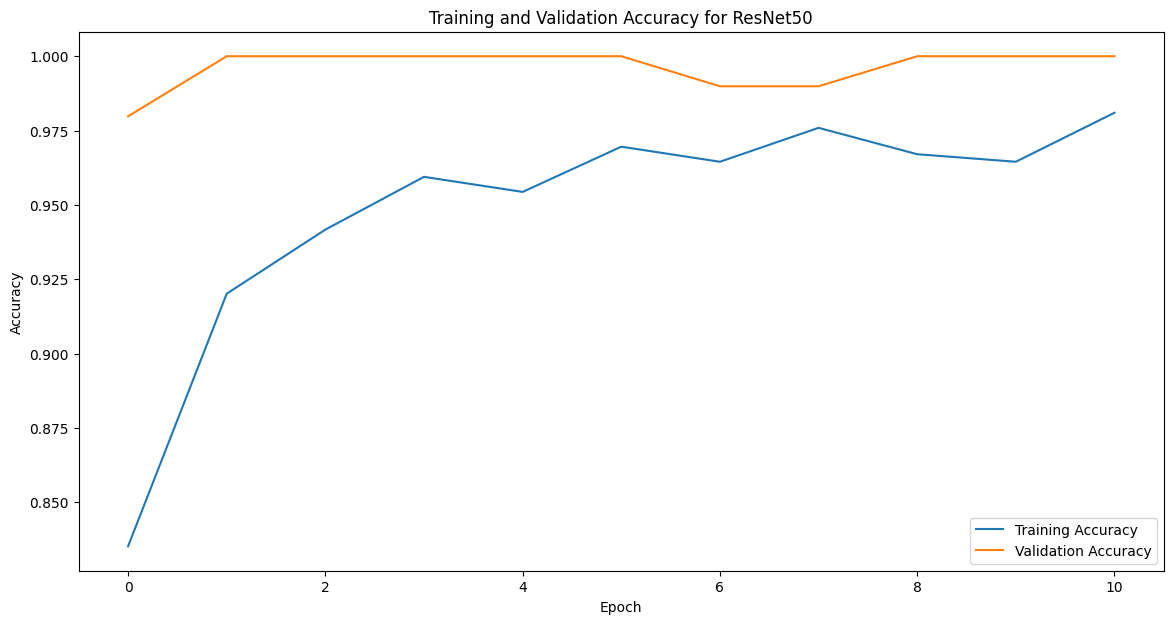
\includegraphics[width=\textwidth]{img/resnet_acc.png} % Replace with actual figure
    \label{fig:resnet_acc}
\end{subfigure}
  \hfill
  % Second image: 2 parts out of 5 (40%)
  \begin{subfigure}[b]{0.8\textwidth}
    \centering
    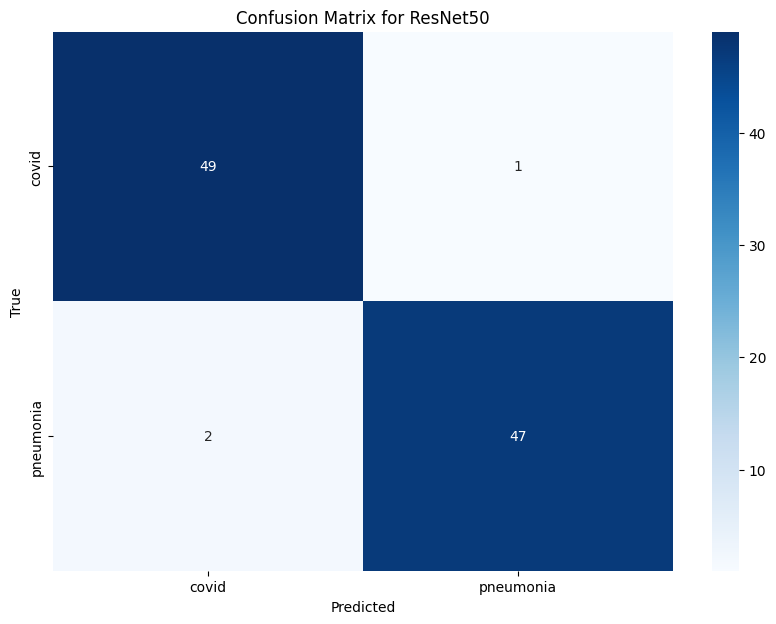
\includegraphics[width=\linewidth]{img/resnet_conf.png}
    \label{fig:resnet_conf}
  \end{subfigure}
\caption{Results for ResNet50}
\end{figure}


\textbf{Analysis}: Swin Tiny Transformer achieved the highest scores among all the metrics.

\subsection{Experiment 2: K-Fold Cross-Validation}
Five-fold cross-validation was performed. Table~\ref{tab:kfold} reports mean metrics. The model was trained using 5-fold cross-validation with 5 epochs per fold, and the final model was trained for 10 epochs, yielding the following validation accuracy results for the models:
\begin{itemize}
\item \textbf{ResNet-50}: Achieved a test accuracy of 94\% after 15 epochs.
\item \textbf{VGG16}: Attained a test accuracy of 98\% after 7 epochs.
\item \textbf{Swin Tiny Transformer}: Reached the highest test accuracy of 99.49\% after 5 epochs.
\end{itemize}

\begin{table}[h]
    \centering
    \caption{K-Fold Cross-Validation Results (Mean $\pm$ Std)}
    \label{tab:kfold}
\begin{tabular}{lccccc}
    \toprule
    Model & Validation Accuracy & Precision & Recall & F1-Score \\
    \midrule
    ResNet-50 & 87.3\% ($\pm$ 0.031\%) & 0.95  & 0.95  & 0.95  \\
    VGG16 & 97.7\% ($\pm$ 0.023\%) & 0.99 & 0.99  & 0.99  \\
    Swin Tiny & 97\% ($\pm$ 0.032\%) & 0.969  & 0.969  & 0.969  \\
    \bottomrule
\end{tabular}
\end{table}

\begin{figure}[h]
    \centering
    \includegraphics[width=0.8\textwidth]{example-image} % Replace with actual figure
    \caption{Boxplot of F1-Scores Across Folds}
    \label{fig:boxplot_kfold}
\end{figure}

\textbf{Analysis}: Low variance in VGG16 suggests robust generalization.

\subsection{Experiment 3: Imbalanced Dataset}
The dataset was adjusted to a 10:1 ratio, with Pneumonia being the minority class. 

The architecture of \textbf{Resnet50} and \textbf{VGG16} models was updated to improve performance on the imbalanced dataset by incorporating L2 regularization (0.01) in the Dense layer, applying class weights computed with the 'balanced' method to address class imbalance, and lowering the classification threshold to 0.3 for better handling of the sigmoid output.

The \textbf{Swin Tiny} model architecture was updated to enhance its performance on the imbalanced dataset by incorporating class weights into the training process.
Table \ref{tab:imbalanced} reports mean metrics.
\begin{itemize}
\item \textbf{ResNet-50}: Achieved a test accuracy of 89.09\% after 10 epochs.
\item \textbf{VGG16}: Reached the highest test accuracy of 98.18\% after 5 epochs.
\item \textbf{Swin Tiny Transformer}: Attained a test accuracy of 97.41\% after 10 epochs.  
\end{itemize}

\begin{table}[h]
    \centering
    \caption{Imbalanced Dataset Results}
    \label{tab:imbalanced}
    \begin{tabular}{lcccc}
        \toprule
        Model & Validation Accuracy & Precision & Recall & F1-Score \\
        \midrule
        ResNet-50 & 92.73\% ($\pm$1.90\%) & 0.89 & 0.87 & 0.83 \\
        VGG16 & 85.91\% ($\pm$10.95\%) & 0.98 & 0.98 & 0.98 \\
        Swin Tiny & 91.74\% ($\pm$3.34\%) & 0.67 & 0.67 & 0.67 \\
        \bottomrule
    \end{tabular}
\end{table}

\textbf{Analysis}: VGG16 excelled in test performance, while ResNet-50 and Swin Tiny showed strong validation results but struggled with minority class balance.


\subsection{Experiment 4: Grayscale Image Classification}
Images were converted to grayscale. Results are presented in Table~\ref{tab:grayscale}.

\begin{table}[h]
    \centering
    \caption{Grayscale Experiment Results}
    \label{tab:grayscale}
    \begin{tabular}{lccccc}
        \toprule
        Model & Accuracy & Precision & Recall & F1-Score & AUC-ROC \\
        \midrule
        ResNet-50 & [X] & [X] & [X] & [X] & [X] \\
        VGG16 & [X] & [X] & [X] & [X] & [X] \\
        Swin Tiny & [X] & [X] & [X] & [X] & [X] \\
        \bottomrule
    \end{tabular}
\end{table}

\textbf{Analysis}: Grayscale conversion [improved/degraded] performance, possibly due to [reason].

\section{Comparison of Results}
\label{sec:comparison}
Table~\ref{tab:comparison} summarizes F1-scores across experiments.

\begin{table}[h]
    \centering
    \caption{Comparison of F1-Scores Across Experiments}
    \label{tab:comparison}
    \begin{tabular}{lcccc}
        \toprule
        Model & Baseline & Imbalanced & K-Fold & Grayscale \\
        \midrule
        ResNet-50 & [X] & [X] & [X] & [X] \\
        VGG16 & [X] & [X] & [X] & [X] \\
        Swin Tiny & [X] & [X] & [X] & [X] \\
        \bottomrule
    \end{tabular}
\end{table}

\begin{figure}[h]
    \centering
    \includegraphics[width=0.8\textwidth]{example-image} % Replace with actual figure
    \caption{Comparison of F1-Scores Across Experiments}
    \label{fig:comparison}
\end{figure}

\textbf{Observations}:
\begin{itemize}
    \item [Model] consistently outperformed others, especially in [experiment].
    \item Imbalanced datasets posed challenges for [model].
    \item Grayscale images [improved/degraded] performance due to [reason].
\end{itemize}

\section{Discussion}
\label{sec:discussion}
The results indicate that [model] is best suited for LUS classification, likely due to [reason]. The imbalanced dataset highlighted the need for techniques like weighted loss. Grayscale images [simplified/reduced] feature extraction, affecting performance. Compared to prior work \cite{cite}, our study provides novel insights into [aspect].

Challenges included [e.g., limited dataset size]. Future work could explore ensemble models or larger datasets to enhance performance.

\section{Conclusion}
\label{sec:conclusion}
This project evaluated ResNet-50, VGG16, and Swin Tiny Transformer for LUS image classification, achieving [key result]. The findings underscore the potential of deep learning in medical imaging and pave the way for improved diagnostic tools.

\begin{thebibliography}{9}
	\bibitem{vafaeezadeh} Vafaeezadeh, M., Behnam, H., \& Gifani, P. (2024). Ultrasound Image Analysis with Vision Transformers—Review. Diagnostics, 14(5), 542. https://doi.org/10.3390/diagnostics14050542
	\bibitem{diaz} Diaz-Escobar, Julia, et al. "Deep-learning based detection of COVID-19 using lung ultrasound imagery." Plos one 16.8 (2021): e0255886.
	\bibitem{mascarenhas} Mascarenhas, Sheldon, and Mukul Agarwal. "A comparison between VGG16, VGG19 and ResNet50 architecture frameworks for Image Classification." 2021 International conference on disruptive technologies for multi-disciplinary research and applications (CENTCON). Vol. 1. IEEE, 2021.
	\bibitem{dosovitskiy} Dosovitskiy, Alexey, et al. "An image is worth 16x16 words: Transformers for image recognition at scale." arXiv preprint arXiv:2010.11929 (2020).
	\bibitem{liu} Liu, Ze, et al. "Swin transformer: Hierarchical vision transformer using shifted windows." Proceedings of the IEEE/CVF international conference on computer vision. 2021.
	\bibitem{perera} Perera, Shehan, Srikar Adhikari, and Alper Yilmaz. "Pocformer: A lightweight transformer architecture for detection of covid-19 using point of care ultrasound." 2021 IEEE international conference on image processing (ICIP). IEEE, 2021.
	\bibitem{xing} Xing, Wenyu, et al. "Frame-to-video-based Semi-supervised Lung Ultrasound Scoring Model." 2023 IEEE International Ultrasonics Symposium (IUS). IEEE, 2023.
	\bibitem{tyagi} Tyagi, Khushal, et al. "Detecting pneumonia using vision transformer and comparing with other techniques." 2021 5th international conference on electronics, communication and aerospace technology (ICECA). IEEE, 2021.
	\bibitem{touvron} Touvron, Hugo, et al. "Training data-efficient image transformers \& distillation through attention." International conference on machine learning. PMLR, 2021.
	\bibitem{he} He, Kaiming, et al. "Deep residual learning for image recognition." Proceedings of the IEEE conference on computer vision and pattern recognition. 2016.
	\bibitem{simonyan} Simonyan, Karen, and Andrew Zisserman. "Very deep convolutional networks for large-scale image recognition." arXiv preprint arXiv:1409.1556 (2014).
\end{thebibliography}





\end{document}